\documentclass[12pt,letter]{aastex}
\usepackage[hyphens]{url}
%\usepackage[breaklinks]{hyperref}   %This is the key package which allows url wrapping.
%\usepackage[draft]{hyperref}
%\usepackage[hyphenbreaks]{breakurl}
\usepackage{longtable}
\usepackage{amsmath,amssymb,multirow,dcolumn,fancyhdr,charter,graphicx}
\usepackage{graphics}
\usepackage{xspace}
\usepackage{color,ulem,epstopdf}
\newcommand{\x}{\sout}
\newcommand{\w}{\color{red}}
\newcommand{\vdag}{(v)^\dagger}
\def\memohr#1{\color{blue}$HR[${\bf #1}$]$ \color{black}}
\def\memoas#1{\color{red}$AS[${\bf #1}$]$ \color{black}}
\def\commentas#1{\color{purple}$AS[${\bf #1}$]$ \color{black}}
\def\refr#1{{\bf #1}}
\usepackage{tikz}
\def\checkmark{\tikz\fill[scale=0.4](0,.35) -- (.25,0) -- (1,.7) -- (.25,.15) -- cycle;} 

%commands
\newcommand{\reb}{{\sc \tt REBOUND}\xspace}
\newcommand{\whfast}{{\sc \tt WHFAST}\xspace}
\newcommand{\ias}{{\sc \tt IAS15}\xspace}
\newcommand{\emcee}{{\sc \tt EMCEE}\xspace}
\newcommand{\Lagr}{\mathcal{L}}
\newcommand{\kep}{{\it Kepler}\xspace}

%journal abbreviations
      
\date{Draft version: \today}

\begin{document}
\section{Introduction}

Proposed sections in the introduction:
\begin{enumerate}
\item Exoplanet detection -- Dominant detection methods (Transit, RV), basic statistics of exoplanets discovered by Kepler Space Telescope.
\item Planet Formation -- MMSN, Core accretion/GI models, Planetesimal Formation, Nice Model. 
\item Planet Dynamics -- Mean Motion Resonance, (planetesimal and gas) Migration, Stability.
\item Numerical Integration -- Hamiltonian Dynamics, integrator types (hybrid, symplectic, high order), coordinate systems (jacobi, heliocentric, whds).
\end{enumerate}

\textbf{Below I am going to elaborate on Planet Dynamics. }

\section{Planet Dynamics}
\subsection{Mean Motion Resonance (MMR)}
\label{sec:MMR}
MMR occurs when the orbital period of one planet is an integer ratio of another. 
Like other types of resonances occuring in nature, MMR results in the amplitude growth of various quantities characterizing the system, like eccentricity, semi-major axis and the longitude of pericentre \citep{SSD1999}. 
As a result, the presence of MMR can strongly affect the formation, evolution and longterm stability of planetary systems in a diversity of ways.
For example, Kirkwood gaps are unstable regions in the asteroid belt carved by MMRs with Jupiter, while Pluto and Neptune are protected from going unstable due to a 3:2 MMR. 

For every $p:q$ MMR (where $p$ and $q$ are integers) there are two important resonant angles:
\begin{align*}
\begin{split}
\phi_1 &= p\lambda_1 - q\lambda_2 + \varpi_1 \\
\phi_2 &= p\lambda_1 - q\lambda_2 + \varpi_2 
\end{split}
\end{align*}
where $\lambda$ is the mean longitude and $\varpi$ is the longitude of periapse. 
For planets to be in MMR, the time variation of one or both of these resonant arguments must be zero.
%, however there are exceptions to this rule.
%For example, planets with commensurate period ratios are not required to be in MMR, and planets a few percent away from period commensurability can be found to be in MMR \citep[e.g.][]{Lee2002}. 
%In addition, circulating resonant angles can be associated with planets in MMR while librating resonant angles can be associated with planets not in MMR \citep{Delisle2012}.
%As a result, it can be difficult to constrain the formation histories of discovered planetary systems. 

\begin{figure}
\centering
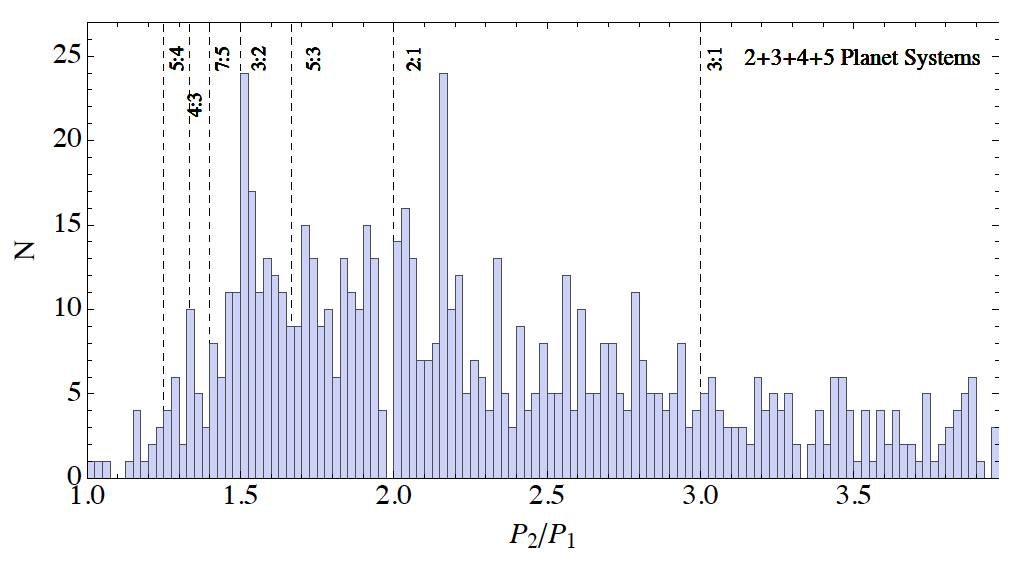
\includegraphics[width=1.00\textwidth]{Figures/KeplerPeriods.png}
\caption{
\footnotesize Period ratios of Kepler planets, image from \citet{Goldreich2014}.}
\label{fig:KepMMR}
\end{figure}

The strength of a given MMR is related to its width, which in turn is related to the order of the resonance ($= p - q$)  and the magnitude of $p$ and $q$ \citep{SSD1999}. 
The lower $p$, $q$ and the order are the stronger the resonance \citep{SSD1999}, making the 2:1 and 3:2 MMRs the most probable resonant locations in nature. 
Figure~\ref{fig:KepMMR} shows the distribution of period ratios for planets discovered by \kep, along with the locations of first and second order MMRs. 
As can be seen, statistical excesses of planets exist near the 2:1 and 3:2 MMR \citep{Lissauer2011,Fabrycky2014,Steffen2015}, supporting the idea that these resonant locations are most capable of trapping planets.

However, the planets from these statistical pileups are typically a few percent away from exact period commensurability, and dissipative mechanisms have been proposed to transport these planets from exact MMR. 
The most popular of these mechanisms are tidal \citep{LithwickWu2012, Batygin2013, Delisle2014}, protoplanetary \citep{Rein2012b, Baruteau2013, Goldreich2014}, and planetesimal \citep{Moore2013, Chatterjee2015}. 
The formation implications for each mechanism are different, and no clear consensus has yet emerged.

%Structure of MMR -- pendulum model, Separatrix, libration of resonant angles. 
%With the exception of a these statistically significant excesses at first order resonances, the period distribution of planets is to first order uniform.

\subsection{Migration}
\subsubsection{Planetesimal-Driven Migration}
Planetesimals passing through the Hill sphere of a planet will exchange angular momentum via gravitational interaction \citep{Ida2000, Kirsh2009}.
If there is an asymmetry to the number of planetesimals interacting with the planet on its near and far sides, a net force will migrate the planet. 
However, to guarantee migration, planetesimal orbits must decouple from the planet. 
A massive enough planet (e.g. Jupiter) will directly eject planetesimals from the system, however if the planet is smaller (e.g. Neptune) planetesimals must decouple by interacting with a neighbouring planet. 
In addition, for sustained migration the planet must constantly encounter fresh, dynamically cold planetesimals \citep{Armitage2010}.  

It is believed that such planetesimal migration occurred for Neptune, migrating outwards into the Kuiper belt and shepherding planetesimals inwards to Jupiter, which subsequently ejected them from the Solar System \citep{Fernandez1984}.
This idea is well supported by observations of the outer Solar System, which show that Pluto, along with a host of smaller bodies, orbit in stable 3:2 MMRs with Neptune \citep{Malhotra1993, Malhotra1995}.

\subsubsection{Gas-Driven migration}
A planet embedded in a protoplanetary disk can migrate via an exchange of angular momentum from disk-planet torques \citep{Goldreich1980}.
Since the discovery of the first hot Jupiter \citep{Mayor1995}, gas-driven migration is believed to play an important role in shaping exoplanetary systems \citep{Lin1996}.
Planet migration comes in two main flavours, Type I and Type II. 

Type I migration occurs when low-mass planets are fully embedded in a protoplanetary disk and do not significantly perturb the disk structure \citep{Armitage2010}. 
At particular resonant locations, known as ``Linblad resonances'', density waves are excited due to gravitational interactions between the planet and disk \citep{Goldreich1979}. 
These density waves exchange angular momentum with the planet, and migration occurs when the inner and outer disk interact asymmetrically with the planet \citep{Goldreich1979}.

Type II migration occurs when high-mass Jovian planets significantly modify the structure of the surrounding protoplanetary disk. 
In particular, a gap is created in the disk by the planet, which in turn locks the planet in place \citep{Armitage2010}.
The planet then migrates inwards at the same rate as the local disk due to ordinary viscous evolution \citep{Armitage2010}.  

In comparison to planetesimal migration, gas-driven migration is still not well understood. 
In particular, standard calculations of gas-driven migration are too quick by an order of magnitude \citep{Lin1986, Tanaka2002}, causing planets to spiral into their central stars before the protoplanetary disk has dispersed.
In contrast with these standard calculations, recent work \citep{Fung2017} has suggested that planets actually do not migrate that much and tend to be better behaved than originally believed. 
A consensus on migration has yet to be established, but it is clear that some form of migration occurs in the universe due to the large number of planets in or near MMR \citep{Lissauer2011,Fabrycky2014,Steffen2015}.

\subsection{Stability}
Although longterm stability of planetary orbits has been studied for hundreds of years by the likes of Newton, Lagrange and Gauss, historically it has been difficult to make progress due to the chaotic and non-integrable nature of planetary systems.  
This chaos is caused by overlapping resonances \citep{Chirikov1979, Lecar2001}, resulting in the divergence of near-identical systems on long timescales. 
However, with the aid of computers the equations of motion governing planetary systems can be brute-force integrated into the future or past with N-body simulation, allowing scientists to answer fundamental questions that have plagued humans for hundreds of years. 
For example, it is now known that the Solar System is marginally stable \citep{Sussman1988, Laskar1994, Lecar2001}, with Mercury having a 1\% chance of colliding with Venus or the sun within a couple billion years \citep{Laskar2009}.
It is also now well established that most known multi-planet systems are packed to capacity, and adding additional planets into these systems would result in dynamical instabilities \citep{Fang2013,Pu2015}.

Although most planetary systems cannot be analytically solved, constraints on these systems can still be derived using analytical means.
For example, \citet{Wisdom1980} and \citet{Duncan1989} showed that for small eccentricities in the Restricted 3-Body Problem, chaotic orbits (leading to close encounters, collisions and ejections) occur when the perturber and particle are separated by $\Delta a \le 1.3\mu_p^{2/7}a_p$ (where subscript $p$ indicates the perturber). 
\citet{Gladman1993} also showed that two massive planets separated by $\Delta a \ge 3.46 R_H$ (where $R_H$ is the mutual Hill radius) are Hill stable, and close encounters are forbidden for all time. 

Since the discovery of numerous exoplanetary systems via \kep, longterm stability has become a popular way to constrain the orbital parameters of that system \citep{Lissauer2011, Steffen2013, Jontof-Hutter2014, Tamayo2015}. 
If one assumes that an observed system is stable over billions of years, grids of N-body integrations can be used to find the stable regions of parameter space, further narrowing the range of possible parameters constrained by observations. 
Although this brute-force method is useful it is not without its costs. 
A typical 10 billion year integration or the Solar System can take weeks to complete, and due to the chaotic nature of planetary systems, hundreds to thousands of realizations must typically be simulated to acquire statistically rigorous answers. 

\bibliographystyle{apj}
\bibliography{intro_ver1.bib}

\end{document}

